\documentclass[UTF8,a4paper,11pt]{ctexart}
\usepackage[margin=2.3cm]{geometry}
\usepackage{amsmath,amssymb,booktabs,graphicx,hyperref,xcolor}
\usepackage{float}
\hypersetup{colorlinks=true,linkcolor=blue,urlcolor=blue}
\graphicspath{{../../../units/task1_numpy_nn_framework/results/}}
\setlength{\parindent}{2em}
\setlength{\parskip}{0.35em}

\title{Task1：NumPy 神经网络框架设计与实验}
\author{WalkerZJH}
\date{2026.06.15 -- 2026.06.21}

\begin{document}
\maketitle

\begin{abstract}
本阶段从零实现一个仅依赖 NumPy 完成模型计算和反向传播的轻量神经网络框架。框架覆盖全连接、卷积、BatchNorm、Dropout、池化、Softmax Cross Entropy 和常用优化器，并通过数值梯度、模式切换与 naive/vectorized 卷积一致性验证实现正确性。在完整 Digits 数据集上完成第一轮正式实验后，进一步在完整 CIFAR-10 上复用相同实验矩阵，对比不同数据复杂度下的模型、学习率及模块行为。实验配置只依据验证集选择，测试集仅用于选择后的最终观察。
\end{abstract}

\section{任务目标与研究问题}

Task1 的实现与 CS231n Assignment 代码相互独立，按核心库、训练器、配置、实验入口和结果归档组织。研究问题包括：手写 backward 是否正确；向量化卷积是否保持一致并提高效率；MLP、MLP+BN 与 CNN 的训练差异；学习率对收敛的影响；BatchNorm 与 Dropout 对拟合和泛化的影响。

\section{数据集与实验协议}

使用 scikit-learn 内置 Digits，共 1797 张 $8\times8$ 灰度图像。像素从 $[0,16]$ 缩放到 $[0,1]$，固定 seed 42 分层划分为训练 1257、验证 269、测试 271。scikit-learn 只负责加载内置数据和分层划分，模型计算与指标均由 NumPy 实现。

正式训练使用完整训练集。统一 baseline 为 hidden dimension 128 的 MLP、Adam、batch size 64、40 epochs、L2 正则 $10^{-4}$。所有 suite 共享数据划分与 seed。按最高 validation accuracy 保存模型状态；test set 在配置选择完成后才计算。

为检验 Digits 接近饱和时结论的区分度，追加完整 CIFAR-10 对照实验。官方训练部分按 seed 42 分层划分为训练 45000、验证 5000，官方测试集保留 10000 张；图像为 $3\times32\times32$，像素缩放到 $[0,1]$。CIFAR-10 沿用 40 epochs、batch size 64、Adam 和同一组模型与消融设置，模型参数采用 float32。配置选择和测试集使用规则与 Digits 一致。

\section{框架设计与模块实现}

\subsection{模块和状态}

\texttt{Parameter} 保存参数与梯度，\texttt{Module} 提供参数、train/eval 递归切换及状态字典。BatchNorm 的 running mean/variance 作为 buffer 一同保存，使 best-validation 快照能够完整恢复推理状态。\texttt{Sequential} 负责顺序执行 forward，并按逆序传播梯度。

\subsection{核心计算}

Linear 使用 $Y=XW+b$，反向为 $dX=dYW^T$、$dW=X^TdY$。ReLU 通过输入正值 mask 传递梯度。Softmax Cross Entropy 对 logits 做最大值平移，并使用 $(p-\mathrm{onehot}(y))/N$ 计算梯度。

卷积同时实现显式循环的 naive 版本和 im2col 版本。向量化 forward 将窗口矩阵与展平卷积核相乘；backward 使用 col2im 和 \texttt{np.add.at} 累加重叠位置梯度。BatchNorm 区分 batch statistics 与 running statistics；Dropout 使用 keep ratio 语义和实例级随机生成器，避免污染 batch shuffle 的随机状态。
\section{正确性与效率验证}

\begin{table}[H]
\centering
\caption{数值梯度检查最大相对误差}
\begin{tabular}{lccc}
\toprule
模块 & $dX$ & $dW/d\gamma$ & $db/d\beta$ \\
\midrule
Linear & $5.58\times10^{-11}$ & $1.69\times10^{-10}$ & $5.27\times10^{-11}$ \\
BatchNorm & $5.93\times10^{-11}$ & $1.54\times10^{-11}$ & $1.45\times10^{-11}$ \\
Conv2D & $8.97\times10^{-9}$ & $2.45\times10^{-9}$ & $5.57\times10^{-11}$ \\
\bottomrule
\end{tabular}
\end{table}

全部误差低于 $10^{-6}$。naive/vectorized 卷积 forward、$dX$、$dW$、$db$ 的最大相对误差低于 $10^{-14}$。当前固定 benchmark 中 naive forward 平均 0.2806 秒，vectorized 平均 0.0009 秒；短时计时存在波动，量级上约为 300 倍加速。Dropout 和 BatchNorm 的 train/eval 行为检查均通过。

\section{Digits Baseline}

Digits 数据集下，MLP baseline 的训练 loss 从 1.9146 降至 0.0508，第 40 个 epoch 的训练准确率为 0.9960、validation accuracy 为 0.9814。选择完成后，test accuracy 为 0.9815。

\begin{figure}[H]
\centering

\includegraphics[width=0.86\textwidth]{baseline/baseline_mlp/training_curves.png}
\caption{Digits 数据集下的 MLP baseline 训练曲线}
\end{figure}

\section{Digits 模型对比}

\begin{table}[H]
\centering
\caption{Digits 数据集下的模型对比（按各模型最高 validation accuracy 记录）}
\begin{tabular}{lrrrrr}
\toprule
模型 & 参数量 & 最佳 epoch & 训练 acc & 验证 acc & 时间/秒 \\
\midrule
MLP & 9610 & 40 & 0.9960 & \textbf{0.9814} & 0.59 \\
MLP+BN & 9866 & 37 & 1.0000 & \textbf{0.9814} & 0.75 \\
CNN & 8986 & 39 & 0.9960 & 0.9777 & 2.62 \\
\bottomrule
\end{tabular}
\end{table}

Digits 数据集下，MLP+BN 的前期收敛更快，并以 0.0869 的 validation loss 达到与 MLP 相同的最高准确率。CNN 在当前 $8\times8$ 输入和单卷积结构下未超过 MLP，NumPy 卷积训练耗时约为 MLP 的 4.4 倍。

\begin{figure}[H]
\centering

\includegraphics[width=0.72\textwidth]{model_comparison/validation_accuracy_comparison.png}
\caption{Digits 数据集下 MLP、MLP+BN 与 CNN 的最佳验证准确率}
\end{figure}

\section{Digits 学习率搜索}

\begin{table}[H]
\centering
\caption{Digits 数据集下固定其他条件后的学习率搜索}
\begin{tabular}{rrrrr}
\toprule
学习率 & 最佳 epoch & 训练 acc & 验证 acc & 验证 loss \\
\midrule
0.0005 & 34 & 0.9753 & 0.9628 & 0.2053 \\
0.0010 & 40 & 0.9960 & 0.9814 & 0.1166 \\
0.0030 & 26 & 0.9992 & \textbf{0.9851} & 0.0936 \\
\bottomrule
\end{tabular}
\end{table}

Digits 数据集下，0.0005 在 40 epochs 内尚未充分收敛；0.003 更快进入高准确率区间且未发散。按 validation accuracy 选中 0.003 后，test accuracy 为 0.9815。

\begin{figure}[H]
\centering

\includegraphics[width=0.72\textwidth]{hparam_tuning/validation_accuracy_comparison.png}
\caption{Digits 数据集下学习率搜索的最佳验证准确率}
\end{figure}

\section{Digits BatchNorm / Dropout 消融}

\begin{table}[H]
\centering
\caption{Digits 数据集下固定 seed 和训练设置后的模块消融}
\begin{tabular}{lrrrr}
\toprule
配置 & 最佳 epoch & 训练 acc & 验证 acc & 验证 loss \\
\midrule
Plain MLP & 40 & 0.9960 & 0.9814 & 0.1166 \\
+ BatchNorm & 37 & 1.0000 & 0.9814 & \textbf{0.0869} \\
+ Dropout ($q=0.8$) & 40 & 0.9928 & \textbf{0.9851} & 0.1208 \\
\bottomrule
\end{tabular}
\end{table}

Digits 数据集下，BatchNorm 改善收敛与 validation loss，但没有提高最高 accuracy。Dropout 降低训练准确率，并在验证集上多正确约一个样本；按验证集选中后，其 test accuracy 为 0.9742，低于 baseline。269 张验证集的 accuracy 最小步长约为 0.0037，因此当前单次划分不足以证明 Dropout 稳定提升，需要多 seed 结果支持。实验仍保留既定选择，不依据 test 回退配置。

\begin{figure}[H]
\centering
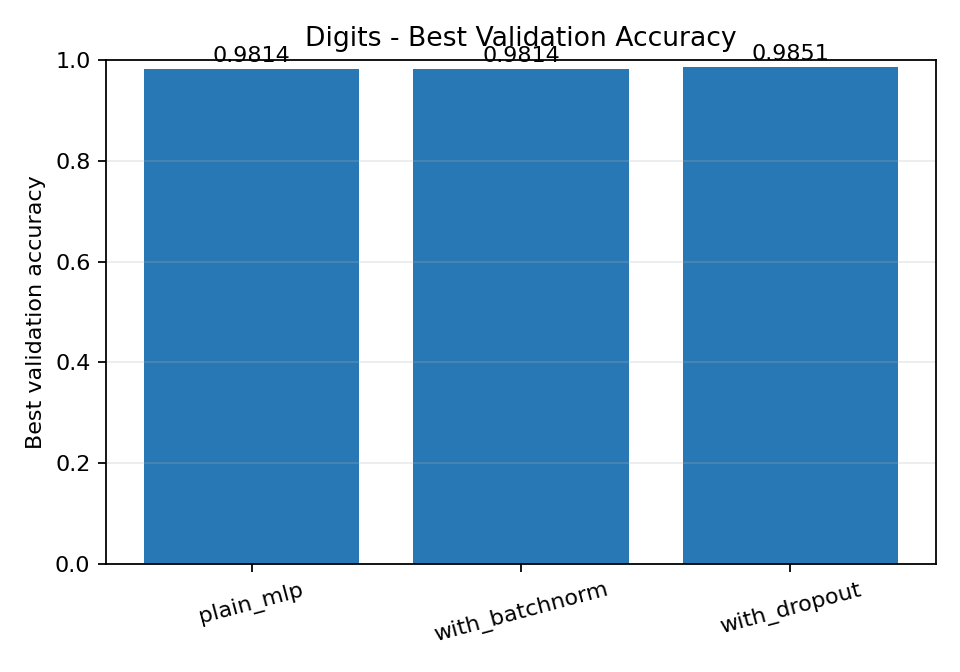
\includegraphics[width=0.72\textwidth]{ablation/validation_accuracy_comparison.png}
\caption{Digits 数据集下 BatchNorm / Dropout 消融的最佳验证准确率}
\end{figure}

\section{完整 CIFAR-10 对照实验}

\subsection{Baseline 与模型对比}

MLP baseline 在第 25 个 epoch 取得最高 validation accuracy 0.4648，此时训练准确率为 0.4880；完成验证集选择后，test accuracy 为 0.4627。相较于 Digits，CIFAR-10 上的准确率分布不再接近饱和，模型结构之间出现了更清晰的差异。

\begin{figure}[H]
\centering

\includegraphics[width=0.86\textwidth]{cifar10_full/baseline/baseline_mlp/training_curves.png}
\caption{CIFAR-10 数据集下的 MLP baseline 训练曲线}
\end{figure}

CIFAR-10 MLP baseline 的训练与验证指标在前期同步改善，中后期验证 loss 和 accuracy 出现波动，训练集仍保持更高准确率。第 25 个 epoch 的 best-validation 快照避免了直接使用最后一轮状态。

\begin{table}[H]
\centering
\caption{完整 CIFAR-10 上的模型对比}
\begin{tabular}{lrrrrr}
\toprule
模型 & 参数量 & 最佳 epoch & 训练 acc & 验证 acc & 验证 loss \\
\midrule
MLP & 394634 & 25 & 0.4880 & 0.4648 & 1.5628 \\
MLP+BN & 394890 & 14 & 0.6278 & 0.5060 & 1.4301 \\
CNN & 132010 & 22 & 0.7403 & \textbf{0.6250} & \textbf{1.1306} \\
\bottomrule
\end{tabular}
\end{table}

CNN 以更少参数取得最高 validation accuracy 0.6250，选中后的 test accuracy 为 0.6089。该结果与 Digits 上 CNN 未超过 MLP 的现象形成对照：当输入扩大到彩色 $32\times32$ 图像后，局部连接与权重共享带来的结构优势更容易体现。MLP+BN 也由 0.4648 提升至 0.5060，说明归一化对当前 MLP 的优化具有实际影响。

\begin{figure}[H]
\centering

\includegraphics[width=0.86\textwidth]{cifar10_full/model_comparison/cnn/training_curves.png}
\caption{CIFAR-10 数据集下验证集选中 CNN 的训练曲线}
\end{figure}

CIFAR-10 CNN 在约第 22 个 epoch 后训练 loss 继续下降、训练准确率继续上升，但 validation loss 转为上升且 validation accuracy 维持在约 0.60 附近，形成明确的泛化差距。因此表中的 CNN 指标来自第 22 个 epoch 的验证集最优状态，而不是第 40 个 epoch。

\begin{figure}[H]
\centering

\includegraphics[width=0.72\textwidth]{cifar10_full/model_comparison/validation_accuracy_comparison.png}
\caption{完整 CIFAR-10 上的模型最佳验证准确率}
\end{figure}

\subsection{学习率搜索}

\begin{table}[H]
\centering
\caption{完整 CIFAR-10 上的 MLP 学习率搜索}
\begin{tabular}{rrrrr}
\toprule
学习率 & 最佳 epoch & 训练 acc & 验证 acc & 验证 loss \\
\midrule
0.0005 & 34 & 0.5487 & \textbf{0.4980} & \textbf{1.4517} \\
0.0010 & 25 & 0.4880 & 0.4648 & 1.5628 \\
0.0030 & 34 & 0.4328 & 0.4164 & 1.6549 \\
\bottomrule
\end{tabular}
\end{table}

验证集选择了 learning rate 0.0005，选中后的 test accuracy 为 0.4931。Digits 上较优的 0.003 在 CIFAR-10 上反而最低，说明学习率结论依赖数据分布、输入维度和损失地形，不能直接跨数据集迁移。

\begin{figure}[H]
\centering

\includegraphics[width=0.72\textwidth]{cifar10_full/hparam_tuning/validation_accuracy_comparison.png}
\caption{完整 CIFAR-10 上不同学习率的最佳验证准确率}
\end{figure}

\subsection{BatchNorm / Dropout 消融}

模块消融固定使用 baseline 训练设置，目的是比较模块影响；学习率搜索结果不与模块消融组合为新的配置。因此，表 7 中 Plain MLP 使用 learning rate 0.001，而不是学习率搜索选中的 0.0005。

\begin{table}[H]
\centering
\caption{完整 CIFAR-10 上的模块消融}
\begin{tabular}{lrrrr}
\toprule
配置 & 最佳 epoch & 训练 acc & 验证 acc & 验证 loss \\
\midrule
Plain MLP & 25 & 0.4880 & 0.4648 & 1.5628 \\
+ BatchNorm & 14 & 0.6278 & \textbf{0.5060} & \textbf{1.4301} \\
+ Dropout ($q=0.8$) & 35 & 0.3900 & 0.3826 & 1.7310 \\
\bottomrule
\end{tabular}
\end{table}

BatchNorm 在验证准确率和 validation loss 上均优于 plain MLP，选中后的 test accuracy 为 0.5085。Dropout keep ratio 0.8 在当前 40-epoch 设置下同时降低训练与验证表现，表现为明显的优化不足；它没有复现 Digits 上单次划分中的轻微验证优势。当前结果只支持该配置在此训练预算下不合适，Dropout 强度和学习率仍需联合控制变量实验。

\begin{figure}[H]
\centering

\includegraphics[width=0.72\textwidth]{cifar10_full/ablation/validation_accuracy_comparison.png}
\caption{完整 CIFAR-10 上的 BatchNorm / Dropout 消融}
\end{figure}

\section{调试过程}

实现过程中修正了配置层级读取和 CSV 字段一致性问题。第一次探索运行还发现不同 run 使用不同 seed 会破坏控制变量，因此该批结果被废弃；正式模型对比、学习率搜索和消融均在固定 seed 后重跑。Dropout 使用实例级 Generator，避免每次 forward 重置全局随机状态。

\section{结论与后续}

Task1 已形成可复现的 NumPy 框架和正式实验闭环。Digits 实验验证了实现正确性，但接近饱和的准确率限制了结构比较的区分度；在完整 CIFAR-10 对照实验中，CNN 明显优于 MLP，BatchNorm 改善 MLP，而学习率和 Dropout 结论不能从 Digits 直接迁移。后续适合补充多 seed 均值与标准差，并对 CNN 的通道数、学习率和正则强度做控制变量搜索。

\end{document}
